\chapter{Scanner}\label{chap:intro}

\lipsum[1]{}

\begin{lstlisting}[language=C++,numbers=none,caption=Ein Beispiel Codestück,label=lst:ex1]
String helloWorld = "Hello World";% chktex 18
\end{lstlisting}

\section{Bauen der Anwendung}
\lipsum{}

\begin{figure}[!htb]
    \centering
      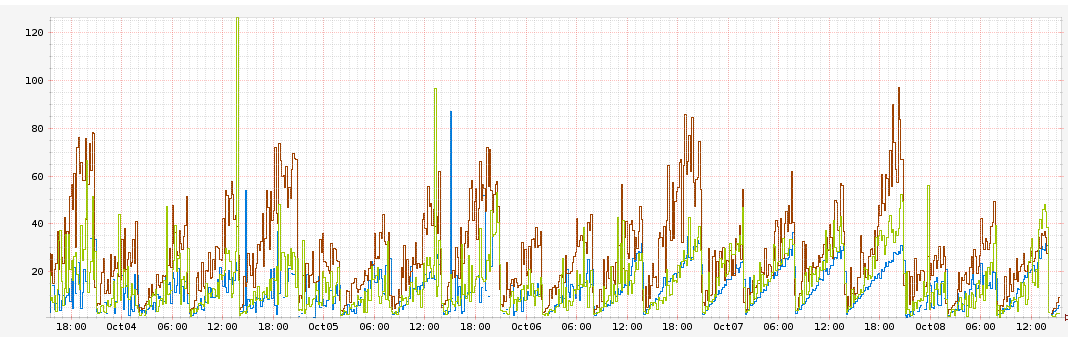
\includegraphics[width=0.85\linewidth]{example-graph.png}
    \caption{Eine Beispielstatistik}{Bildquelle:~\cite{JavaBeginner-Binding}}\label{fig:example}
\end{figure}

\lipsum{}
\section{References}

Literatur:~\cite{Example}

Look at~\ref{sec:objekthierarchie}

Example link to listing~\ref{lst:ex1}

And an example footnote\footnote{Look at this webpage: \url{https://www.google.com}}

\lipsum[2-3]{}% chktex 8
